En esta sección desarrollaremos y mostraremos los resultados de los experimentos para:

\begin{itemize}
\item Los protocolos distinguidos.
\item La incidencia de paquetes ARP en la red.
\item Los nodos distinguidos.
\end{itemize}

\subsection{Experimento protocolos distinguidos}

Para analizar los protocolos distinguidos fuimos guardando los resultados de sniffear diferentes redes y tomar como fuente de información S el campo .type de los paquetes que se fueron procesando. Fundamentalmente vimos tres tipos de protocolos: ARP, IP (es decir IPv4) e IPv6. Dentro de los paquetes IP pudimos ver que la mayoría, a su vez, llevaban paquetes ICMP, TCP o UDP. A traves de la libreria "Scapy" de "Python" tomamos dos muestras de los paquetes 'Ethernet' que se pudieron detectar:

\begin{itemize}
\item Dataset 1: Biblioteca pabellon 2 (wifi) a las 3pm
\item Dataset 2: Laboratorios pabellon 1 (wifi) a las 5pm
\end{itemize}

Cada dataset contiene todos los paquetes observados junto al protocolo que se uso. De ahí calculamos la cantidad de apariciones de cada protocolo, la probabilidad de aparición de cada protocolo, calculamos la entropía y la comparamos con la información que aporta cada símbolo de S (ARP, IP e IPv6).\\

Por eso, para distinguir \emph{protocolos} tomamos a
aquellos cuya probabilidad de aparición era alta, de forma que la información provista por el símbolo fuera menor a la entropía de la fuente S.\\

Ahora, para analizar los datos, planteamos histogramas donde podemos ver la cantidad de información $I(s) = -log_2(P(s))$ que aporta cada símbolo de la fuente. Luego lo comparamos con la entropía y definimos los \emph{protocolos distinguidos} como los que son mas bajos que la entropía. Esto lo hicimos porque según la fórmula de Shannon, la entropía $\sum\limits_{s \in S} P(s) * I(s)$ se corresponde con la información promedio que aporta cada símbolo a la fuente. Por lo cual, los símbolos cuya cantidad de información sea mas baja que la entropía son muy predecibles ya que aparecerán muchas veces y, por ejemplo, si tuviera que asignarle otro símbolo a cada uno de ellos, me convendría representarlos con menos bits para disminuir la longitud promedio del código. \\

Los resultados fueron los siguientes: \\

% Dataset 1 ----------------------------------

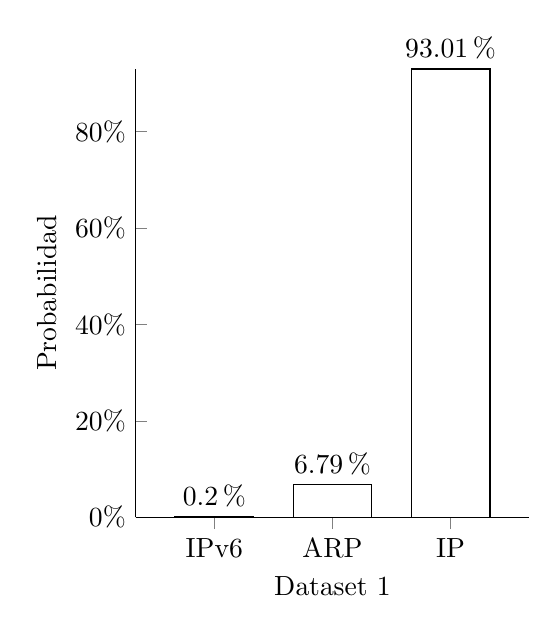
\begin{tikzpicture}
\begin{axis}[
    ybar,
    bar width=1cm, % Width of the bar
    x=1.5cm, % Distance between the centers of the bars
    enlarge x limits={abs=1cm}, % The distance between the center of the first bar and the left edge
    enlarge y limits=false,
    ymin=0,
    xtick=data,
    xlabel= {Dataset 1},
    ylabel= {Probabilidad},
    symbolic x coords={IPv6,ARP,IP},
    point meta={y*100}, %y-Werte mal 100 für Prozent 
    yticklabel={\pgfmathparse{\tick*100}\pgfmathprintnumber{\pgfmathresult}\%},
    axis lines*=left,
    clip=false
    ]
\addplot [
    draw=black,
    fill=white,
    nodes near coords={\pgfmathprintnumber{\pgfplotspointmeta}\,\%},
    error bars/.cd,
        y dir=both,
        y explicit
    ] coordinates{(IPv6,0.001998001998)
        (ARP,0.0679320679321)
        (IP,0.93006993007)};
\end{axis}
\end{tikzpicture}
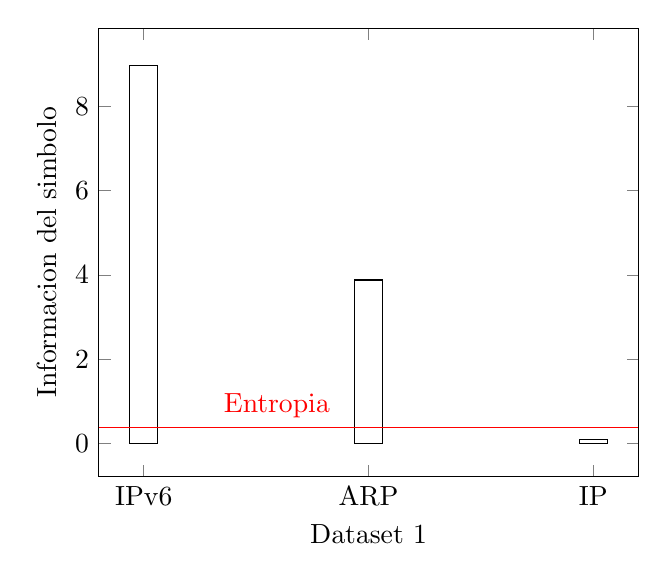
\begin{tikzpicture}
\begin{axis}[
    symbolic x coords={IPv6,ARP,IP},
        ylabel = {Informacion del simbolo},
        xlabel = {Dataset 1},
        xtick=data]
    \addplot[ybar,fill=white] coordinates {
        (IPv6,8.9672262584)
        (ARP,3.8797634179)
        (IP,0.1045889014)
    };
    \draw [red] ({rel axis cs:0,0}|-{axis cs:ARP,0.378751880122}) -- ({rel axis cs:1,0}|-{axis cs:ARP,0.378751880122}) node [pos=0.33, above] {Entropia};
\end{axis}
\end{tikzpicture} \\

% Dataset 2 ----------------------------------

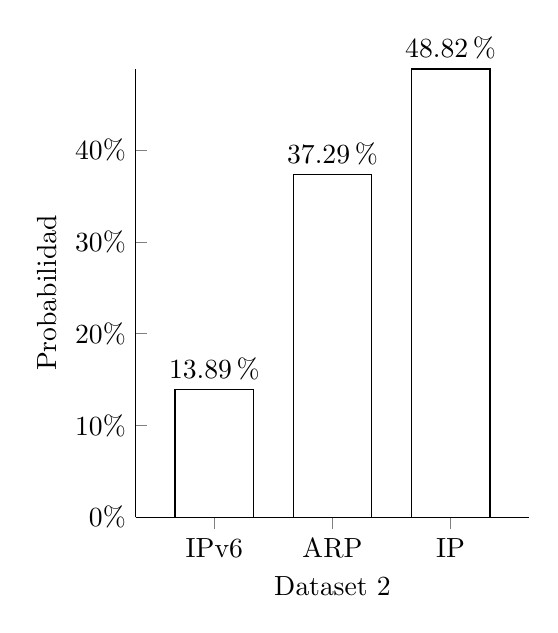
\begin{tikzpicture}
\begin{axis}[
    ybar,
    bar width=1cm, % Width of the bar
    x=1.5cm, % Distance between the centers of the bars
    enlarge x limits={abs=1cm}, % The distance between the center of the first bar and the left edge
    enlarge y limits=false,
    ymin=0,
    xtick=data,
    xlabel= {Dataset 2},
    ylabel= {Probabilidad},
    symbolic x coords={IPv6,ARP,IP},
    point meta={y*100}, %y-Werte mal 100 für Prozent 
    yticklabel={\pgfmathparse{\tick*100}\pgfmathprintnumber{\pgfmathresult}\%},
    axis lines*=left,
    clip=false
    ]
\addplot [
    draw=black,
    fill=white,
    nodes near coords={\pgfmathprintnumber{\pgfplotspointmeta}\,\%},
    error bars/.cd,
        y dir=both,
        y explicit
    ] coordinates{
        (IPv6,0.1389218889)
        (ARP,0.3728838729)
        (IP,0.4881942382)};
\end{axis}
\end{tikzpicture}
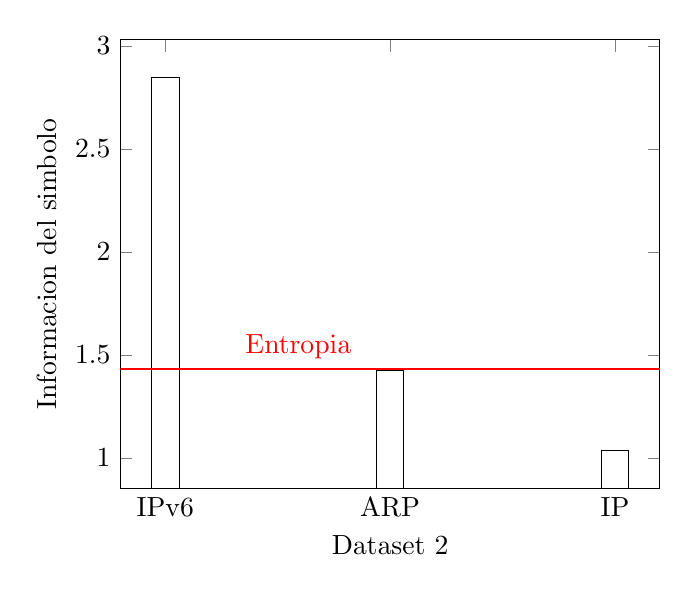
\begin{tikzpicture}
\begin{axis}[
    symbolic x coords={IPv6,ARP,IP},
        ylabel = {Informacion del simbolo},
        xlabel = {Dataset 2},
        xtick=data]
    \addplot[ybar,fill=white] coordinates {
        (IPv6,2.847654163)
        (ARP,1.423201692)
        (IP,1.034472826)
    };
    \draw [red] ({rel axis cs:0,0}|-{axis cs:ARP,1.4313141279}) -- ({rel axis cs:1,0}|-{axis cs:ARP,1.4313141279}) node [pos=0.33, above] {Entropia};
\end{axis}
\end{tikzpicture} \\

% Discusion ------------------------------------

Por lo que podemos ver, la incidencia de ARP es muy baja en el Dataset 1 ya que en una biblioteca hay poco recambio de dispositivos y pocos hosts, lo cual hace que la incidencia de ARP sea menor. En cambio, si hay muchos mas paquetes IP, lo cual tiene sentido porque es el protocolo que todos los hosts usan para conectarse a internet. Entonces como podemos ver, el único símbolo predecible menor que la entropía es el de IP, el cual es el único protocolo distinguido en este dataset. \\

En el segundo Dataset, ya podemos hablar de una red (el Laboratorio de Computación) en la cual no solamente hay muchos mas hosts, sino el recambio de dispositivos que entran y se van de la red es mayor, por lo cual la incidencia de ARP sube. A su vez, IP sigue siendo el protocolo más usado al igual que en el dataset anterior. Tanto la información que aporta ARP como IP superan la entropía de la fuente de información S, por eso ambos son en este caso protocolos distinguidos. \\
% end subsection

\subsection{Experimento incidencia de ARP}

Para poder observar la incidencia de paqueres ARP en la red voy a utilizar una serie de muestras tomadas de distintas redes y graficarlas en un histograma, despues de mostrar
los resultados daremos una explicación del por que de los mismo.

\begin{figure}[ht!]
\centering
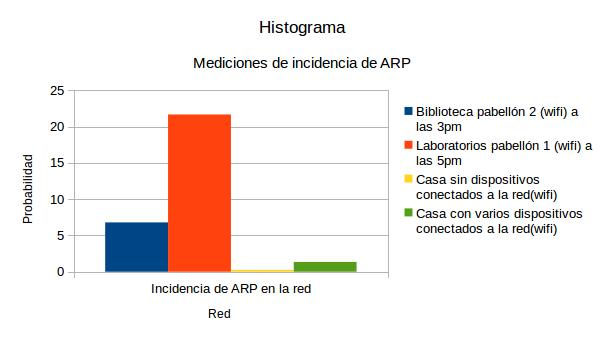
\includegraphics[width=90mm]{imagenes/IncidenciaARP.jpg}
\caption{Comparación de porcentaje de apariciones de ARP en distintas redes o con distintas condiciones.\label{overflow}}
\end{figure}

Como podemos ver la red de los laboratorios tiene más porcentaje de paquetes ARP que el de la biblioteca. Esto se debe a que en el laboratorio del pabellón 1 ingresan 
constantemente personas y, por lo tanto, la mayoría de ellos ingresan en la red a través de las computadoras del mismo o de usando el wifi de estos con sus celulares. Esto 
ocurre en menor medida en la biblioteca ya que no se usan computadoras que no sean propias de los que ingresan, por lo tanto, por la red hay mucho más trafico de paquetes 
ARP en los laboratorios. Además al estar en una red privada, es más común que se efectúen envíos de mensajes entre computadoras y los routers de las mismas.

\begin{comment}
Intento de experimentos1:

Para poder observar la incidencia de paqueres ARP en la red voy a utilizar el buscador de Google Chrome y la función de scapy arping. Usando la interfaz de wlan0 podre sniffear
los paquetes que habra con el buscador y usando arping podre enviar paquetes ARP.\\

Ejecuto  sudo ./capture.py wlan0 entropia-tipos 1000 y, al mismo tiempo, abro el buscador. 

Resultados:

Simbolo 2048 tiene probabilidad 0.996158770807(IP).

Simbolo 34525 tiene probabilidad 0.00128040973111(IPv6).

Simbolo 2054 tiene probabilidad 0.00256081946223(ARP).

La entropia de la fuente es 0.0492085855963.

Simbolo 2048 tiene probabilidad 0.996158770807(IP).

Simbolo 34525 tiene probabilidad 0.00256081946223(IPv6).

Simbolo 2054 tiene probabilidad 0.00128040973111(ARP).

La entropia de la fuente es 0.0398813035719.

Simbolo 2048 tiene probabilidad 0.99875(IP).

Simbolo 2054 tiene probabilidad 0.00125(ARP).

La entropia de la fuente es 0.0138570614629.

Simbolo 2048 tiene probabilidad 0.998740554156(IP).

Simbolo 2054 tiene probabilidad 0.00125944584383(ARP).

La entropia de la fuente es 0.013948087353.

Simbolo 2048 tiene probabilidad 0.985987261146(IP).

Simbolo 34525 tiene probabilidad 0.0101910828025(IPv6).

Simbolo 2054 tiene probabilidad 0.00382165605096(ARP).

La entropia de la fuente es 0.118197558737.

Ejecuto  sudo ./capture.py wlan0 entropia-tipos 100 y, al mismo tiempo, ejecuto arping("192.168.2.0/24").

Resultados:
Simbolo 2048 tiene probabilidad 0.0481481481481(IP).

Simbolo 2054 tiene probabilidad 0.951851851852(ARP).

La entropia de la fuente es 0.278477724908.

Simbolo 2048 tiene probabilidad 0.0769230769231(IP).

Simbolo 34525 tiene probabilidad 0.0244755244755(IPv6).

Simbolo 2054 tiene probabilidad 0.898601398601(ARP).

La entropia de la fuente es 0.554261234655.

Simbolo 2048 tiene probabilidad 0.0115384615385(IP).

Simbolo 2054 tiene probabilidad 0.988461538462(ARP).

La entropia de la fuente es 0.0908278259323.

Simbolo 2048 tiene probabilidad 0.011320754717(IP).

Simbolo 34525 tiene probabilidad 0.00754716981132(IPv6).

Simbolo 2054 tiene probabilidad 0.981132075472(ARP).

La entropia de la fuente es 0.153356025339.

Simbolo 2054 tiene probabilidad 1.0(ARP).

La entropia de la fuente es 0.0.

Ejecuto  sudo ./capture.py wlan0 entropia-tipos 100 y, al mismo tiempo, abro buscador y ejecuto arping("192.168.2.0/24").

Resultados:

Simbolo 2048 tiene probabilidad 0.737424547284(IP).

Simbolo 34525 tiene probabilidad 0.00201207243461(IPv6).

Simbolo 2054 tiene probabilidad 0.260563380282(ARP).

La entropia de la fuente es 0.847640262877.

Simbolo 2048 tiene probabilidad 0.735412474849(IP).

Simbolo 34525 tiene probabilidad 0.00603621730382(IPv6).

Simbolo 2054 tiene probabilidad 0.258551307847(ARP).

La entropia de la fuente es 0.875119992479.

Simbolo 2048 tiene probabilidad 0.761948529412(IP).

Simbolo 34525 tiene probabilidad 0.00183823529412(IPv6).

Simbolo 2054 tiene probabilidad 0.236213235294(ARP).

La entropia de la fuente es 0.807325191625.

Simbolo 2048 tiene probabilidad 0.757518796992(IP).

Simbolo 34525 tiene probabilidad 0.00093984962406(IPv6).

Simbolo 2054 tiene probabilidad 0.241541353383(ARP).

La entropia de la fuente es 0.808024777478.

Simbolo 2048 tiene probabilidad 0.754066985646(IP).

Simbolo 2054 tiene probabilidad 0.245933014354(ARP).

La entropia de la fuente es 0.804768238572.


Ejecuto  sudo ./capture.py wlan0 entropia-tipos 100 y, al mismo tiempo, arping("192.168.2.0/24") y arping("10.4.2.0/27").
\end{comment}

% end subsection
